\section{Experiments}
\label{sec:experiments}

We evaluate whether reliability-aware reward scaling can substantially reduce OPD training cost while preserving downstream reasoning accuracy.
Beyond final benchmark accuracy and training time, we measure local student-teacher dynamics on student-visited states, including overlap ratio, top-$p$ acceptance, and effective reliable length.

\subsection{Experimental Setup}

\noindent\textbf{Training data.}
We train on DAPO-Math-17K \citep{yu2025dapo}, following the OPD setting used in recent reasoning experiments.
Training prompts are shuffled before each run.
The primary RL outcome reward is final-answer correctness. However, OPD supplies dense token-level distillation rewards.

\noindent\textbf{Models.}
We evaluate five teacher-student pairs to test the reliability signal across distinct OPD dynamics.
DeepSeek-R1-Distill-Qwen-1.5B is distilled from DeepSeek-R1-Distill-Qwen-7B, a larger same-family reasoning model whose higher benchmark score may not imply locally exploitable token-level feedback \citep{guo2025deepseek}.
The same student is also distilled from JustRL-DeepSeek-1.5B, a same-size RL-improved teacher obtained from DeepSeek-R1-Distill-Qwen-1.5B \citep{he2025justrl}.
Qwen3-1.7B-Base and Qwen3-4B-Base are distilled from Qwen3-4B (Non-thinking), isolating how a thinking-mode shift interacts with student scale within the same model family \citep{yang2025qwen3}.
Finally, DeepSeek-R1-Distill-Qwen-7B is distilled from Skywork-OR1-7B, providing a high-initial-overlap setting where \method~is expected to preserve long-context supervision rather than shorten the rollout.
Together, these combinations test the same claim under different conditions: the controller reduces computation when reliability decays, while preserving dense supervision when compatibility remains high.

\noindent\textbf{Baselines.}
We compare baseline OPD, fixed-length truncation baselines, and \method~variants.
Fixed-length OPD uses the same distillation objective as baseline OPD but clamps the maximum response length to a fixed budget.
Random pruning matches either the retained token fraction or retained OPD reward mass of \method~while choosing pruned positions independently of student-teacher compatibility.
These controls test whether the benefit comes from the student-teacher compatibility signal rather than from generic shorter rollouts or lower reward density.
The main \method~configuration uses overlap ratio with threshold $\gamma=0.7$.
We also report a teacher top-$p$ action-acceptance variant with $p=0.95$. Both variants use top-$k=16$, $w_{\mathrm{drop}}=0.01$, $w_{\mathrm{base}}=0.5$, and dynamic-length hit ratio $0.1$.
Unless otherwise stated, dynamic response length uses initial 2048, min 1024, max 12288, update step 100, margin 100, and shrink patience 3.

\noindent\textbf{Evaluation.}
We evaluate on AMC23, AIME24, AIME25, HMMT24, and HMMT25.
The primary metric is pass@1 accuracy under a fixed evaluation protocol.
We also report relative training time reduction, response-length statistics, overlap ratio, top-$p$ acceptance rate, and effective reliable length.
Training time is measured relative to baseline OPD under the same student-teacher pair.

\subsection{Main Results}

\begin{table*}[t]
    % \vspace{3mm}
    \centering
    \small
    \renewcommand\arraystretch{1.2}
    \setlength{\tabcolsep}{5pt}
    \caption{Main results for \method. Accuracy is reported in percent. Time reduction is relative to baseline OPD under the same student-teacher pair.}
    \label{tab:main-results}
    \begin{tabular}{l|c|c|c|c|c|c|c}
       \toprule
       \textbf{Method} & \textbf{AMC23} & \textbf{AIME24} & \textbf{AIME25} & \textbf{HMMT24} & \textbf{HMMT25} & \textbf{Time} & \textbf{Red.} \\
       \midrule
       \rowcolor{gray!10} \multicolumn{8}{c}{\textit{DeepSeek-R1-Distill-Qwen-1.5B / JustRL-DeepSeek-1.5B}} \\
       \opd~& 77.5 & 43.5 & 32.7 & \textbf{23.5} & 18.1 & 6.9h & 0\% \\
       \opd{} (Truncate 4k) & 77.8 & 43.1 & 31.0 & 22.7 & 17.9 & 4.8h & 30.4\% \\
       \rowcolor[HTML]{EDF5F5}\textbf{\method{} (top-$p$)} & 77.3 & 44.0 & 30.8 & 23.3 & \textbf{19.8} & \textbf{4.3h} & \textbf{37.7\%} \\
       \rowcolor[HTML]{D7E8E8}\textbf{\method{} (overlap)} & \textbf{78.4} & \textbf{45.2} & \textbf{33.5} & 22.7 & 18.8 & \textbf{4.1h} & \textbf{40.6\%} \\
       \midrule
       \rowcolor{gray!10} \multicolumn{8}{c}{\textit{DeepSeek-R1-Distill-Qwen-1.5B / DeepSeek-R1-Distill-Qwen-7B}} \\
       \opd~& \textbf{66.4} & \textbf{33.5} & 25.4 & 14.4 & \textbf{15.0} & 12.5h & 0\% \\
       \opd{} (Truncate 4k) & 66.3 & 31.7 & \textbf{25.8} & 14.2 & 14.4 & 6.6h & 47.2\% \\
       \rowcolor[HTML]{EDF5F5}\textbf{\method{} (top-$p$)} & 65.5 & 29.6 & 24.2 & \textbf{14.6} & 14.0 & 4.8h & 61.6\% \\
       \rowcolor[HTML]{D7E8E8}\textbf{\method{} (overlap)} & 65.9 & 33.3 & \textbf{25.8} & \textbf{14.6} & \textbf{15.0} & \textbf{4.0h} & \textbf{68.0\%} \\
       \midrule
       \rowcolor{gray!10} \multicolumn{8}{c}{\textit{Qwen3-1.7B-Base / Qwen3-4B (Non-thinking)}} \\
       \opd~& 28.0 & \textbf{7.3} & 2.9 & 2.1 & 0.6 & 16.5h & 0\% \\
       \opd{} (Truncate 4k) & 28.6 & 6.3 & 2.9 & 2.3 & \textbf{1.0} & 12.9h & 21.8\% \\
       \rowcolor[HTML]{EDF5F5}\textbf{\method{} (top-$p$)} & 28.4 & 5.6 & 2.9 & 1.9 & 0.6 & 11.5h & 30.3\% \\
       \rowcolor[HTML]{D7E8E8}\textbf{\method{} (overlap)} & \textbf{29.1} & \textbf{7.3} & \textbf{4.2} & \textbf{2.9} & \textbf{1.0} & \textbf{10.3h} & \textbf{37.6\%} \\
       \midrule
       \rowcolor{gray!10} \multicolumn{8}{c}{\textit{Qwen3-4B-Base / Qwen3-4B (Non-thinking)}} \\
       \opd~& \textbf{42.7} & 14.8 & 10.6 & 5.4 & 2.9 & 28.5h & 0\% \\
       \opd{} (Truncate 4k) & 41.9 & 15.2 & 13.5 & 4.8 & 2.7 & 22.3h & 21.8\% \\
       \rowcolor[HTML]{EDF5F5}\textbf{\method{} (top-$p$)} & 40.5 & 13.1 & 12.7 & 4.8 & 4.0 & 20.0h & 29.8\% \\
       \rowcolor[HTML]{D7E8E8}\textbf{\method{} (overlap)} & \textbf{42.7} & \textbf{16.3} & \textbf{14.6} & \textbf{6.7} & \textbf{5.6} & \textbf{13.5h} & \textbf{52.6\%} \\
       \bottomrule
    \end{tabular}
    \vspace{-4mm}
\end{table*}

The main result is a consistent efficiency gain without meaningful degradation in downstream accuracy.
Across the main low-compatibility runs, the overlap-ratio variant reduces training time by 35.7\%, 68.0\%, 37.6\%, and 52.6\%, while benchmark accuracy remains close to the corresponding OPD baseline.
Accuracy differences are mixed across individual benchmarks and should be interpreted as secondary: \method~slightly improves several AIME/HMMT scores, but also decreases a few entries such as AIME24 under the DeepSeek-R1-Distill-Qwen-7B teacher and HMMT24 under the JustRL-DeepSeek-1.5B teacher.
This pattern is consistent with the role of \method~as a reliability-aware efficiency mechanism rather than a standalone accuracy-improvement method.
The top-$p$ action-acceptance variant is generally more conservative and often weaker than overlap, suggesting that exact sampled-token acceptability can be too strict for reasoning traces, whereas candidate-space overlap better captures whether the teacher still supplies exploitable local supervision.



\begin{figure*}[t]
\centering
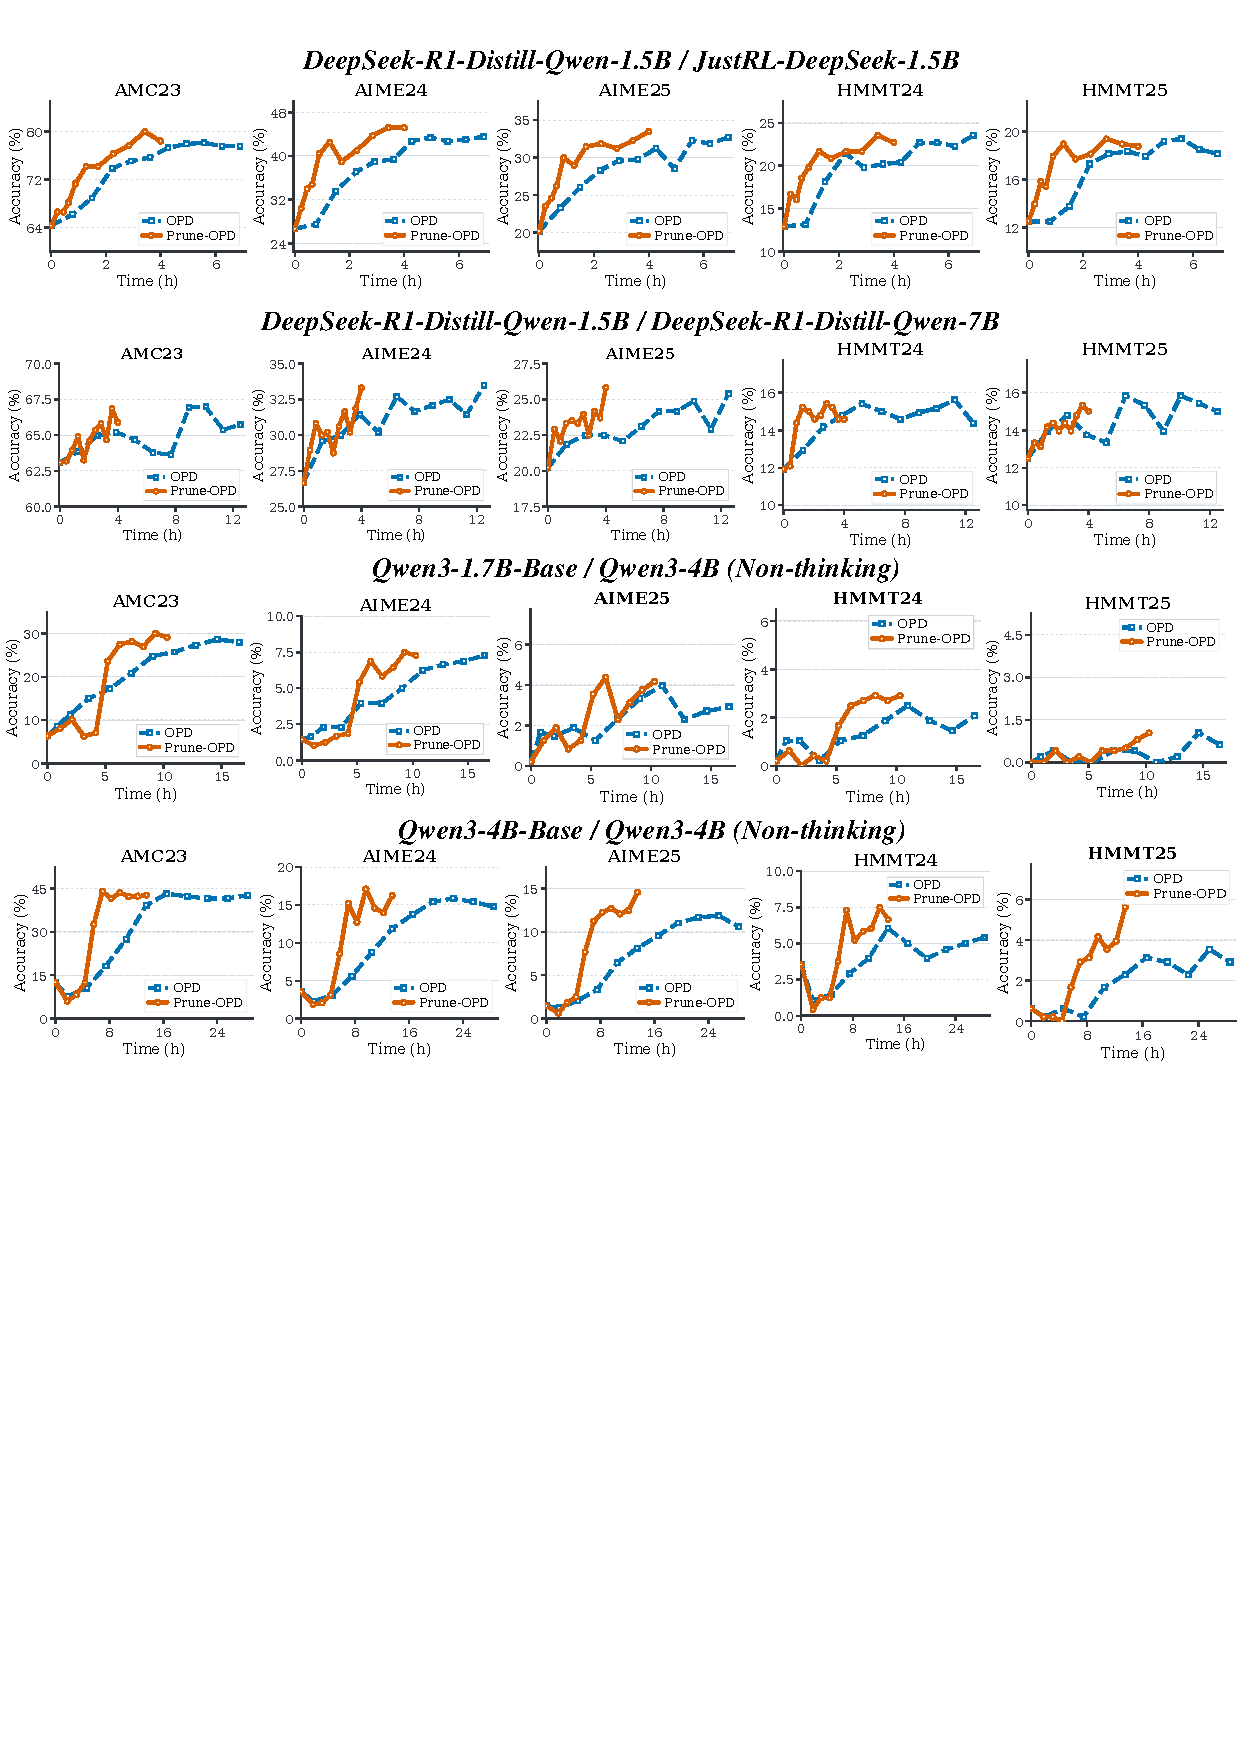
\includegraphics[width=\textwidth]{figs/acc-time-final_compat.pdf}
\vspace{-6mm}
\caption{Accuracy over wall-clock time for the 4 DeepSeek student-teacher pairs. Each panel uses wall-clock time as the x-axis and benchmark accuracy as the y-axis, comparing OPD and \method. A successful curve should match or exceed OPD accuracy while reaching comparable checkpoints earlier in time.}
\label{fig:time-accuracy}
\vspace{-4mm}
\end{figure*}

\subsection{Adaptive Behavior Under High Compatibility}

This setting tests whether \method~uniformly shortens every run.
When the teacher and student have high top-$k$ overlap, the effective-length hit ratio is quickly satisfied and the dynamic controller opens the training window to 12288 tokens.
The resulting training time and accuracy are nearly unchanged from OPD.
Figure~\ref{fig:pair5-high-compatibility-dynamics} should show the corresponding mechanism from three views: the overlap ratio remains high, the dynamic response budget tracks the long reliable context rather than forcing early truncation, and the AMC23 learning curve compares whether \method~matches OPD-level accuracy while avoiding the rigidity of fixed truncation.
This supports the intended interpretation that \method~is an adaptive reliability controller, not a hard length penalty.

\subsection{Training Dynamics}


Figure~\ref{fig:pair1-training-accuracy} examines whether \method~changes the learning dynamics or simply removes rollout computation.
For the JustRL-DeepSeek-1.5B teacher, the benchmark-wise step-accuracy curves should show that \method~follows the same learning trajectory as OPD on AMC23, AIME24, AIME25, HMMT24, and HMMT25, rather than achieving speed by sacrificing accuracy.
Figure~\ref{fig:pair1-training-diagnostics} explains where the saved computation comes from: the weight-by-position plot should show suffix reward attenuation after accumulated prefix drift, the effective-length plot should show the dynamic maximum OPD length adapting to the reliable supervision window, and the overlap-ratio curve should confirm that pruning is driven by the measured local compatibility signal.


\begin{table*}[t]
    \centering
    \small
    \renewcommand\arraystretch{1.2}
    \setlength{\tabcolsep}{5pt}
    \caption{High-compatibility behavior. DeepSeek-R1-Distill-Qwen-7B and Skywork-OR1-7B start with overlap ratio around 0.94.}
    \label{tab:high-compatibility}
    \begin{tabular}{l|c|c|c|c|c|c|c}
       \toprule
       \textbf{Method} & \textbf{AMC23} & \textbf{AIME24} & \textbf{AIME25} & \textbf{HMMT24} & \textbf{HMMT25} & \textbf{Time} & \textbf{Red.} \\
       \midrule
       \rowcolor{gray!10} \multicolumn{8}{c}{\textit{DeepSeek-R1-Distill-Qwen-7B / Skywork-OR1-7B}} \\
       \opd~& 88.3 & \textbf{67.1} & \textbf{52.5} & \textbf{33.5} & \textbf{32.1} & 17.5h & 0\% \\
       \opd{} (Truncate 4k) & \textcolor{red!40}{87.2} & \textcolor{red!40}{66.0} & \textbf{\textcolor{red!40}{48.8}} & \textbf{\textcolor{red!40}{31.0}} & \textcolor{red!40}{30.4} & 11.3h & \textbf{35.4\%} \\
       \rowcolor[HTML]{D7E8E8}\textbf{\method{} (overlap)} & \textbf{88.9} & 66.7 & 52.1 & 33.1 & 31.5 & 17.0h & 2.9\% \\
       \bottomrule
    \end{tabular}
\end{table*}

\begin{figure*}[t]
\vspace{-3mm}
\centering
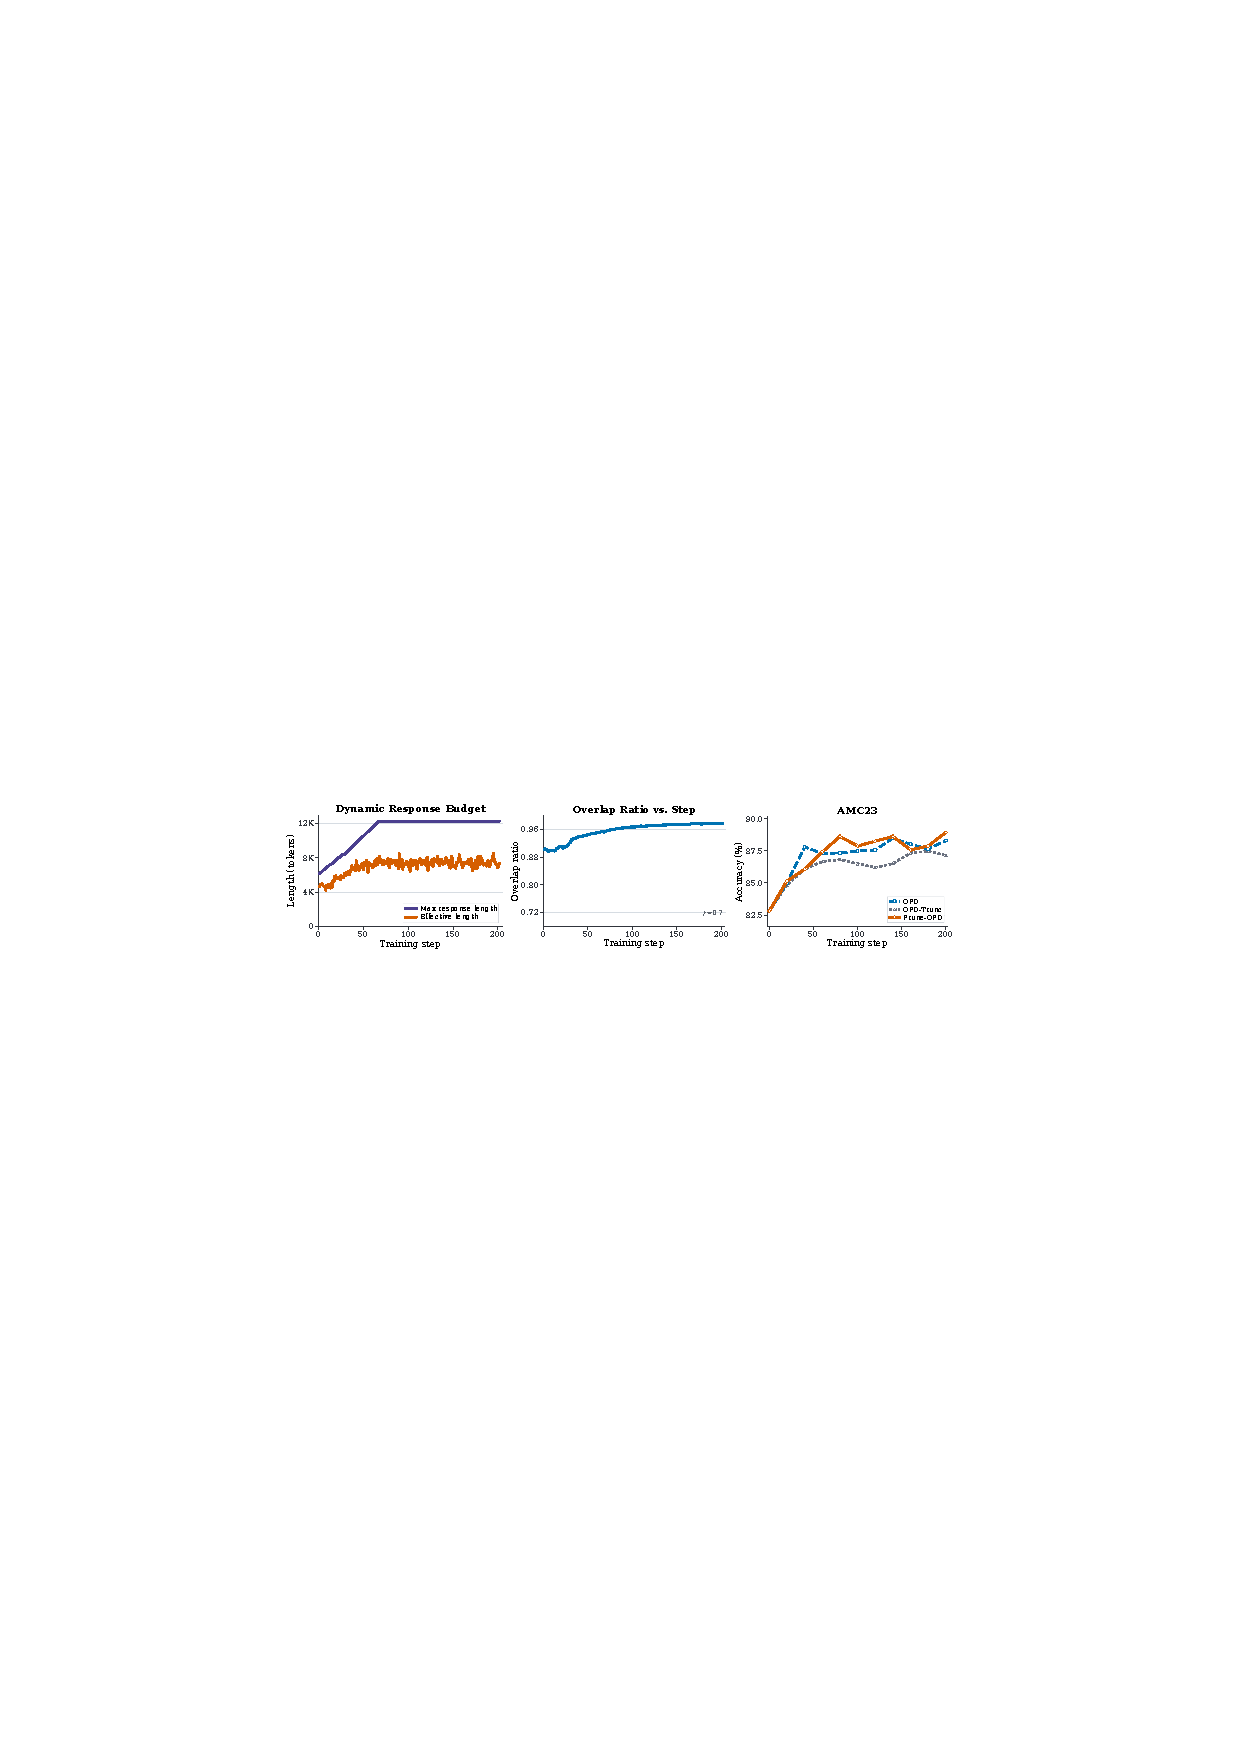
\includegraphics[width=\textwidth]{figs/fig3_compat.pdf}
\vspace{-5mm}
\caption{High-compatibility training dynamics for DeepSeek-R1-Distill-Qwen-7B / Skywork-OR1-7B. Left: effective response length and maximum OPD length versus training step. Middle: overlap ratio versus training step. Right: AMC23 accuracy over training, comparing OPD, \opd{} (Truncate 4k), and \method.}
\label{fig:pair5-high-compatibility-dynamics}
\vspace{-6mm}
\end{figure*}


\begin{figure*}[t]
\centering
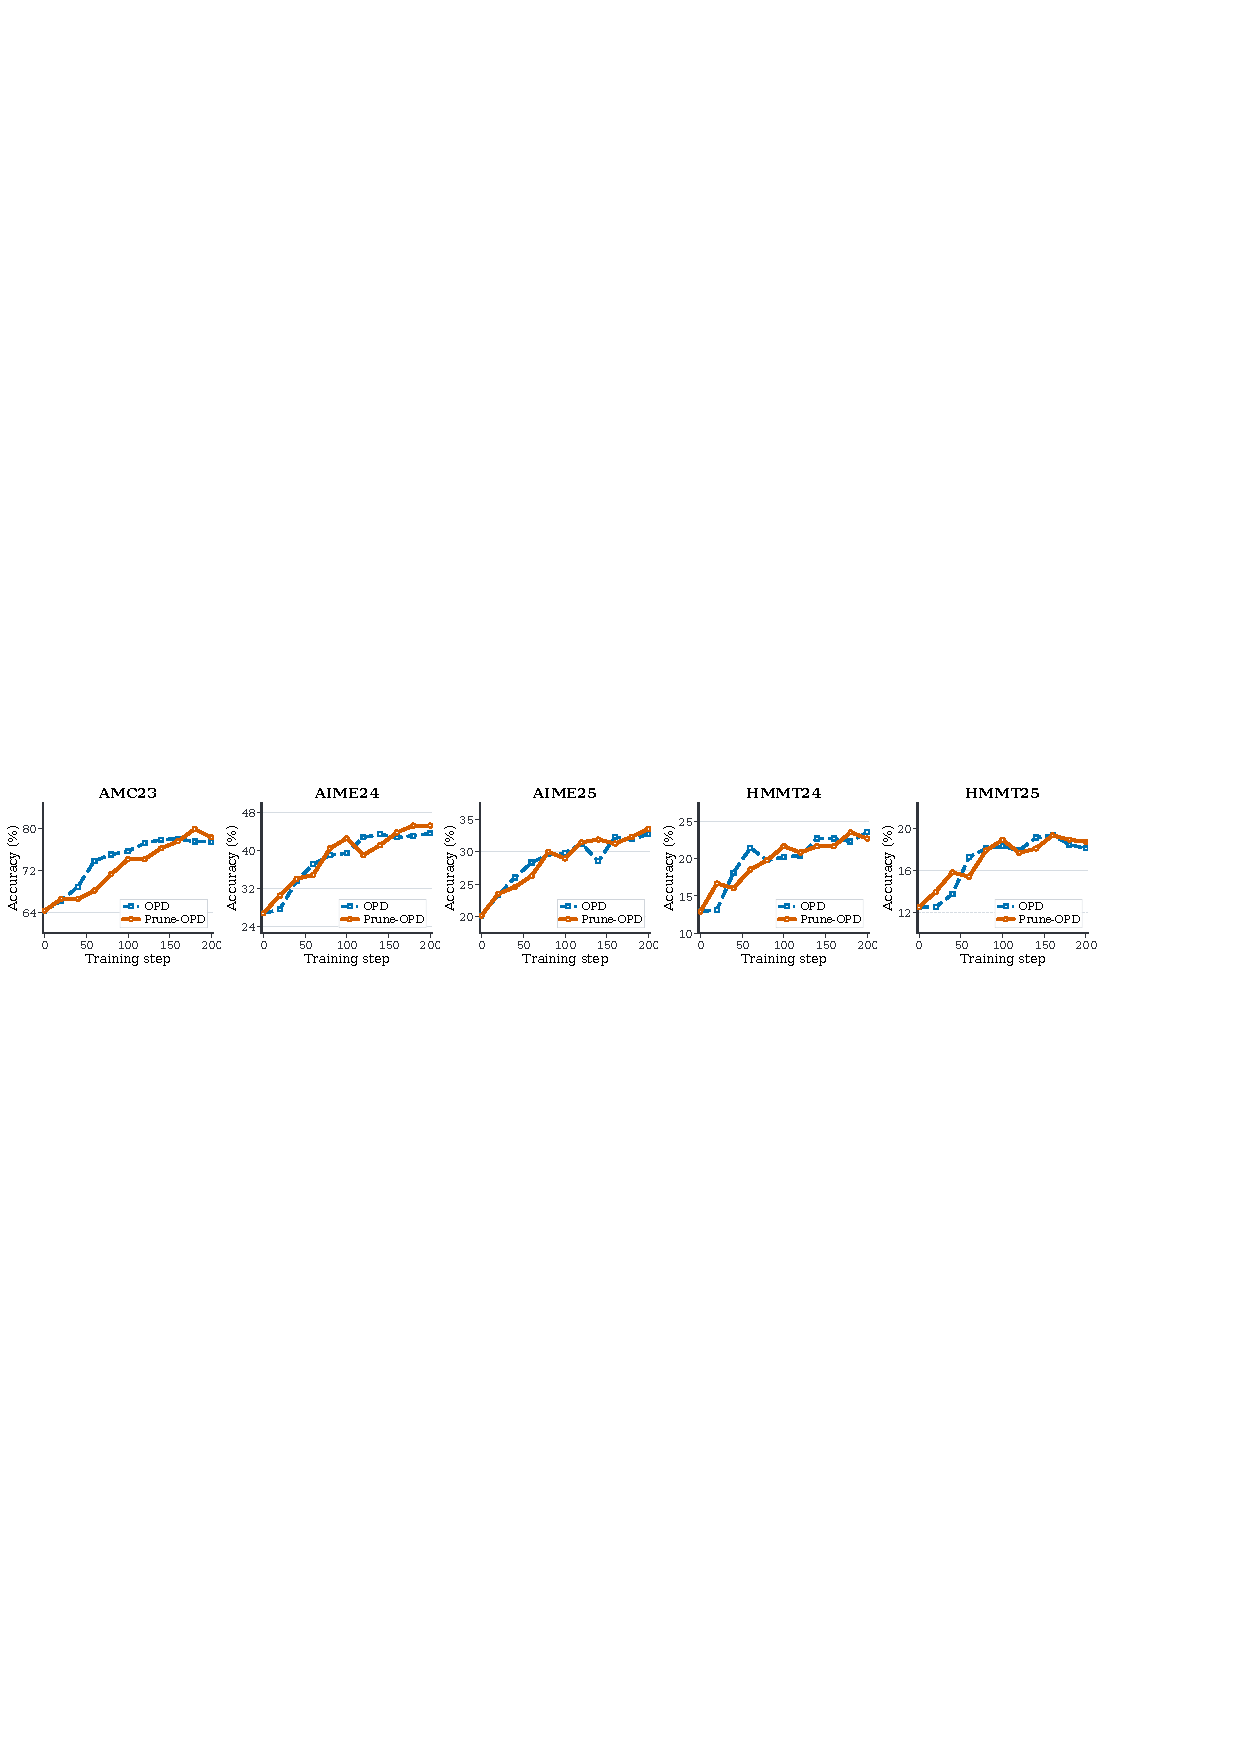
\includegraphics[width=\textwidth]{figs/fig4_compat.pdf}
\vspace{-5mm}
\caption{Training-step accuracy dynamics for DeepSeek-R1-Distill-Qwen-1.5B distilled from JustRL-DeepSeek-1.5B. The five panels report benchmark accuracy over training steps on AMC23, AIME24, AIME25, HMMT24, and HMMT25, comparing OPD and \method.}
\label{fig:pair1-training-accuracy}
\end{figure*}

\begin{figure*}[t]
\vspace{-3mm}
\centering
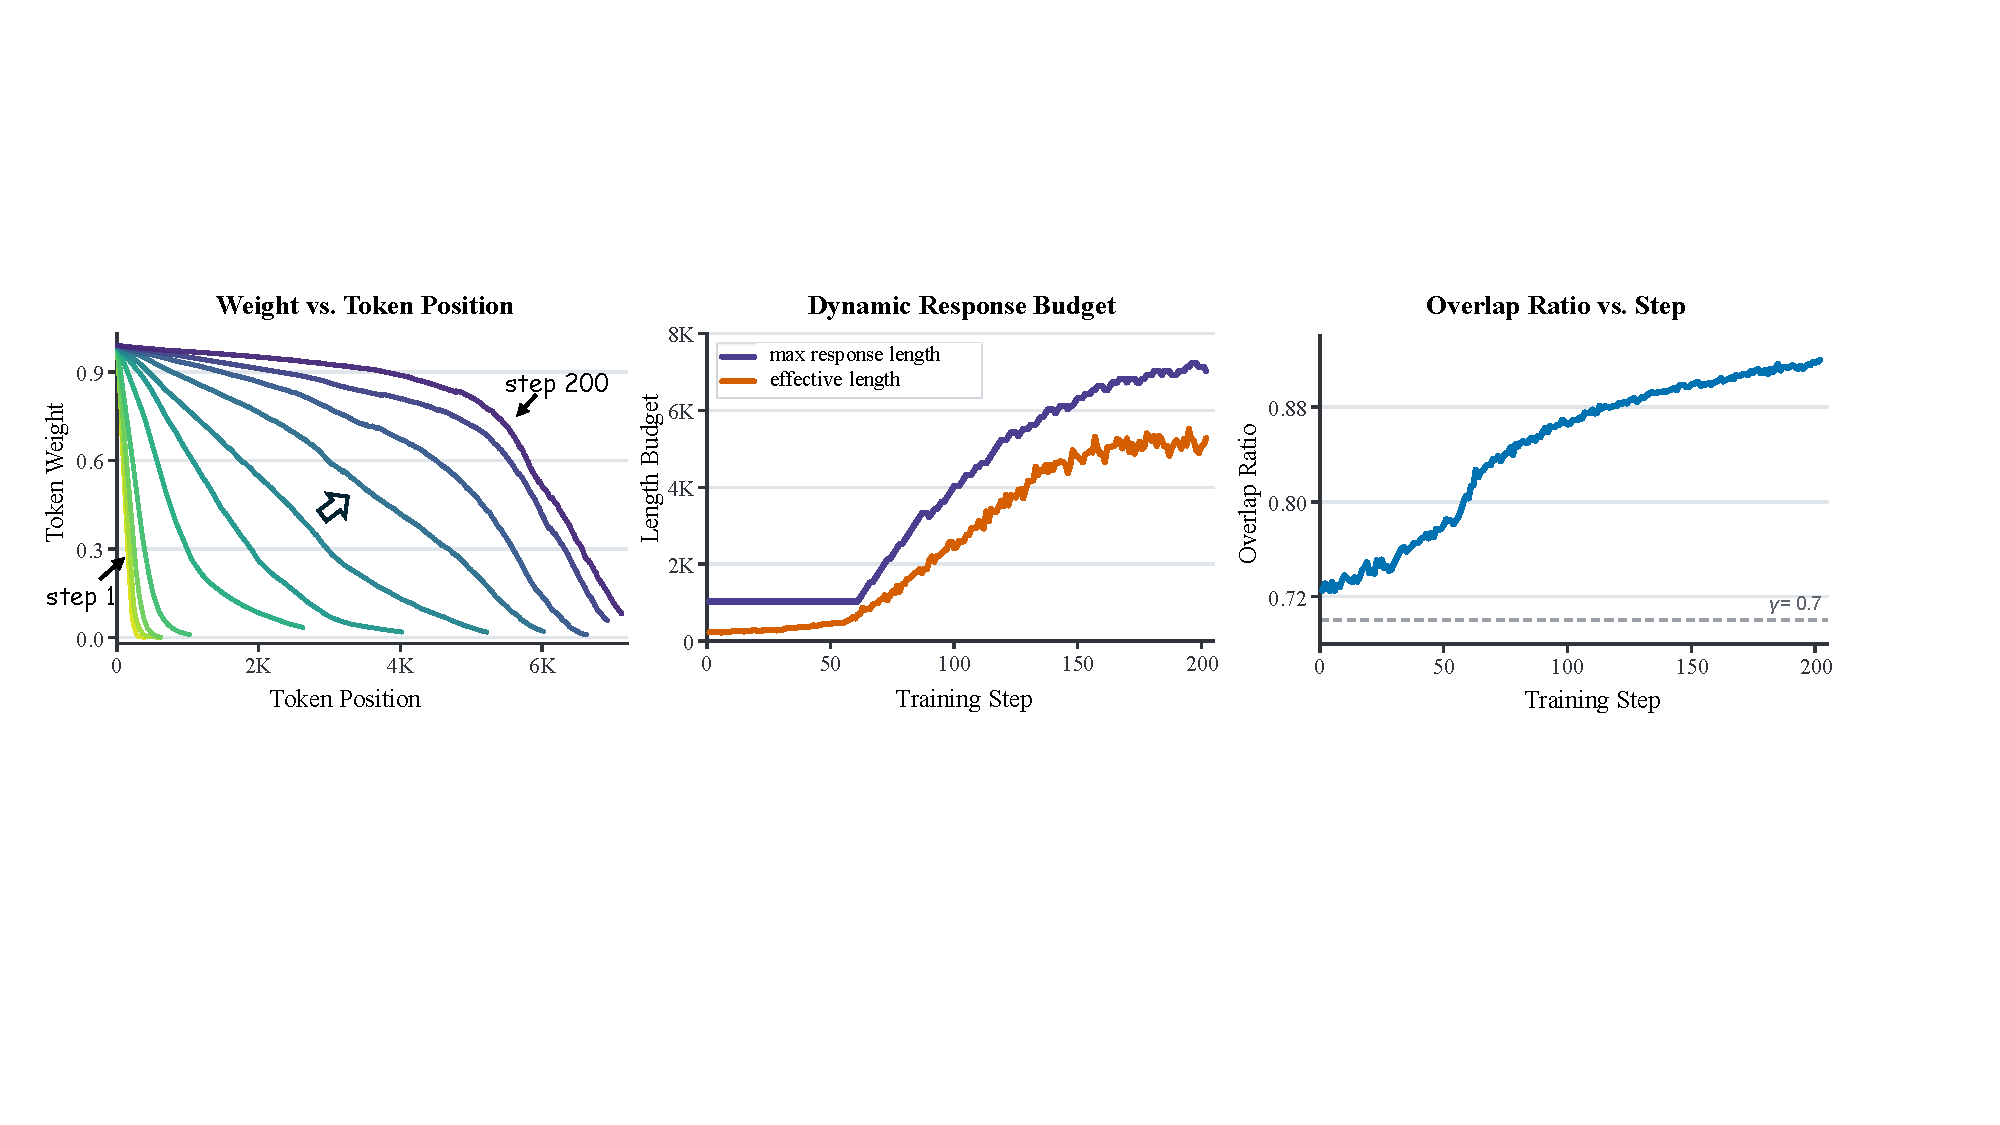
\includegraphics[width=\textwidth]{figs/fig5_compat.pdf}
\vspace{-6mm}
\caption{Training-dynamics diagnostics for DeepSeek-R1-Distill-Qwen-1.5B distilled from JustRL-DeepSeek-1.5B. The panels report mean Prune-OPD weight by token position with curves every 20 training steps from 0 to 200; effective response length and maximum OPD length over training; and overlap ratio over training.}
\label{fig:pair1-training-diagnostics}
\vspace{-4mm}
\end{figure*}



\subsection{Wall-Clock Efficiency}


Figure~\ref{fig:time-accuracy} evaluates the core efficiency claim on the wall-clock axis: \method~should reduce elapsed training time without reducing accuracy, and in some cases can slightly improve it.
If \method~is working as intended, its curves should lie to the left of OPD at comparable accuracy levels, or above OPD at the same wall-clock time.
This presentation directly tests whether \method~reaches OPD-level, and occasionally better, accuracy with less elapsed training time across both DeepSeek teacher-student combinations.
Together with the dynamics in Figures~\ref{fig:pair1-training-accuracy} and~\ref{fig:pair1-training-diagnostics}, these results show that: reliability-aware suffix down-weighting shortens unproductive rollout computation while preserving the useful prefix supervision that drives final performance.


\begin{table}[htbp]
\vspace{-3mm}
\centering
\caption{Overlap-threshold ablation on DeepSeek-R1-Distill-Qwen-1.5B / JustRL-DeepSeek-1.5B. 
% Accuracy is reported in percent.
}
\label{tab:threshold-ablation}
\small
\setlength{\tabcolsep}{4pt}
\renewcommand{\arraystretch}{1.1}
\begin{tabular}{lccccccc}
\toprule
Threshold $\gamma$ & AMC23 & AIME24 & AIME25 & HMMT24 & HMMT25 & Time & Red. \\
\midrule
0.6 & \textbf{78.9} & \textbf{45.4} & 33.1 & 22.0 & \textbf{18.8} & 4.8h & 30.4\%\\
\rowcolor[HTML]{D7E8E8}0.7 & 78.4 & 45.2 & \textbf{33.5} & \textbf{22.7} & \textbf{18.8} & 4.1h & 40.6\% \\
0.8 & 77.8 & 44.5 & 31.5 & 21.9 & 18.0 & 3.1h & 55.1\%\\
0.9 & 76.8 & 43.9 & 30.8 & 21.8 & 17.9 & 2.4h & 65.2\%\\
\bottomrule
\end{tabular}
\vspace{-4mm}
\end{table}

\subsection{Ablation Study}

\noindent\textbf{OPD with simple truncation.}
We include \opd{} (Truncate 4k) as a fixed-budget baseline in Tables~\ref{tab:main-results} and~\ref{tab:high-compatibility}.
This baseline uses the same OPD objective but shortens every rollout uniformly, without observing student-teacher compatibility.
Although simple truncation can reduce cost and may be effective for some teacher-student pairs, it is not a reliable substitute for \method.
In particular, for DeepSeek-R1-Distill-Qwen-1.5B / JustRL-DeepSeek-1.5B and DeepSeek-R1-Distill-Qwen-7B / Skywork-OR1-7B, truncating at a fixed 4K budget degrades performance because it discards useful long-prefix supervision.
This failure mode highlights the limitation of a rigid length rule: it cannot distinguish drifted suffixes from long but still compatible reasoning trajectories.

\noindent\textbf{Pruning metric: overlap ratio vs. top-$p$ acceptance.}
The metric ablation is reported in Table~\ref{tab:main-results}.
Across the completed runs, overlap ratio is the stronger default: it gives equal or larger time reduction than top-$p$ acceptance while generally preserving accuracy better.
We attribute this to its support-level nature: it asks whether student and teacher still share high-probability candidate regions, rather than requiring the sampled student token to fall inside the teacher's visible nucleus.
This makes overlap ratio a smoother reliability signal for long reasoning traces, where multiple locally plausible continuations may remain valid.

% \noindent\textbf{Pruning metric: overlap ratio vs. top-$p$ acceptance.}
% The metric ablation is reported in Table~\ref{tab:main-results}.
% Across the completed runs, overlap ratio is the stronger default: it achieves equal or larger time reduction than top-$p$ acceptance and generally better preserves accuracy.
% The reason is that overlap ratio measures compatibility between the student and teacher high-probability regions, which is exactly the local condition needed for OPD rewards to remain exploitable.
% By contrast, top-$p$ acceptance is an action-level test: it asks whether the sampled student token lies inside the teacher's visible nucleus.
% This can be overly strict for reasoning traces, where multiple locally plausible next tokens may lead to valid continuations even if the exact sampled token is outside the teacher's truncated top-$p$ set.
% Thus, overlap ratio provides a smoother and more robust signal for deciding when to attenuate suffix rewards.

\noindent\textbf{Prune-OPD threshold ablation.}
We ablate the overlap-ratio threshold in Table~\ref{tab:threshold-ablation} on DeepSeek-R1-Distill-Qwen-1.5B / JustRL-DeepSeek-1.5B.
The completed $\gamma=0.7$ setting gives a strong operating point: it preserves OPD-level benchmark performance while reducing training time by 35.7\%.
A lower threshold should be more permissive, producing fewer bad events and longer effective distillation lengths; a higher threshold should prune earlier and may remove useful long reasoning if set too aggressively.
The central conclusion is that $\gamma=0.7$ provides both performance protection and substantial training-efficiency improvement.
